\section{PDF critical path analysis}\label{sec:pdf}


As previously mentioned, the timing analysis of synchronous dataflow is predicated on predictable token consumption/production rates at discrete, globally synchronised points in time. This discrete scheduling may be a global clock transition in hardware implementations or a scheduling time slice in software implementations. On asynchronous dataflow, this discrete abstraction must be abandoned: absolute continuous time must instead be adopted. This is true even in Globally Asynchronous Locally Synchronous (GALS) hardware implementations: even though each actor operates under its own (discrete) clock, clock frequencies may be completely unrelated in frequency and phase. The goal of PDF analysis is to obtain a token throughput timing profile in absolute time, under unpredictable token consumption/production rates. This is done through network profiling, collecting runtime statistics about each actor's behaviour.

\subsection{Single Input Single Output Actors}

\begin{figure}[tb]
  \centering
  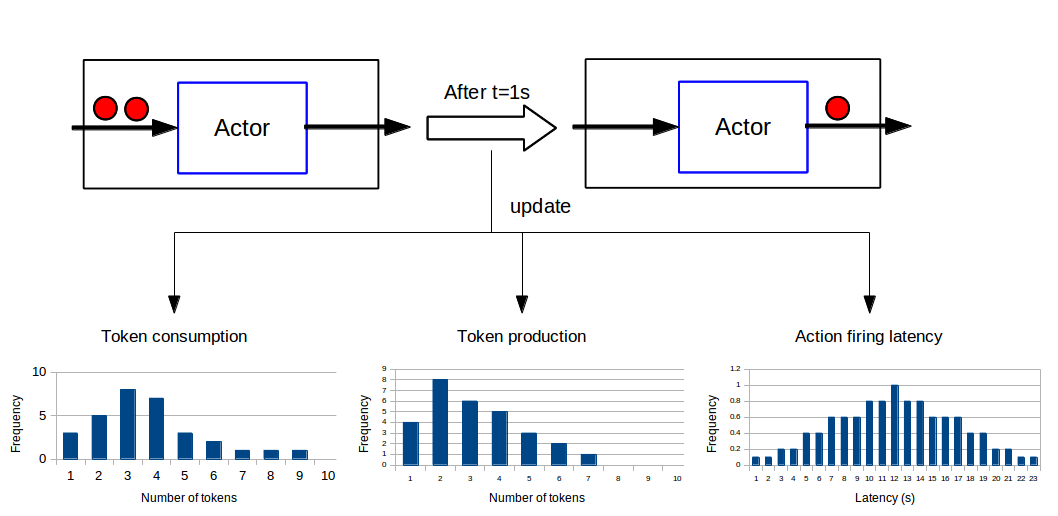
\includegraphics[width=1\columnwidth]{img/example1.png}
  \caption{Profile update after action firing: token consumption is updated by incrementing bin 2, token production is updated by incrementing bin 1, and latency is is updated by incrementing bin 1. Histogram shapes are purely illustrative.}
  \label{fig:example1}
\end{figure}




For the simplest possible dynamic asynchronous actor, with one input and one output port, we monitor how many tokens are consumed and produced per action firing, and how long it takes between successive action firings, assuming sufficient input tokens are always available. It should be noted that we assume these two metrics to be independent: the dynamic nature of actors doen't allow for any assumptions of correlation between token consumption and latency. Fig. \ref{fig:example1} depicts an example of such profiling, for different token throughput and action latencies, and examples of histograms for each metric.



\par In order to model actors' behaviour in absolute continuous time, 

\begin{itemize}
\item each actor latency (avg of actions) as a PDF
\item effect of pipeline analysis of PDF
\item effect of feedback loops analysis of PDFs
\end{itemize}

